	\section{Overview: High-level components and their interaction}
A brief description of the general design context, the general approach and the overall design of the system with its processes is presented in this section of the DD.
Our system will be developed as a 4-tiered JEE application, divided as Client Tier, Web Tier, Business Tier and the EIS Tier. It is distributed between client machines, Java EE server machine and the database.
\\The mobile and web applications in particular are thin since data operations will be computed by a central server; in this way there is no heavy load on user side clients. We think that this is the most feasible approach because the two applications have the same goals. 
\\The diagram below provides a better understanding of the components of our system, highlighting the interactions among them:
%\subsubsection{Architecture Component Diagram}
\begin{figure}[!h]
  \centering
  \vspace{0.2cm}
  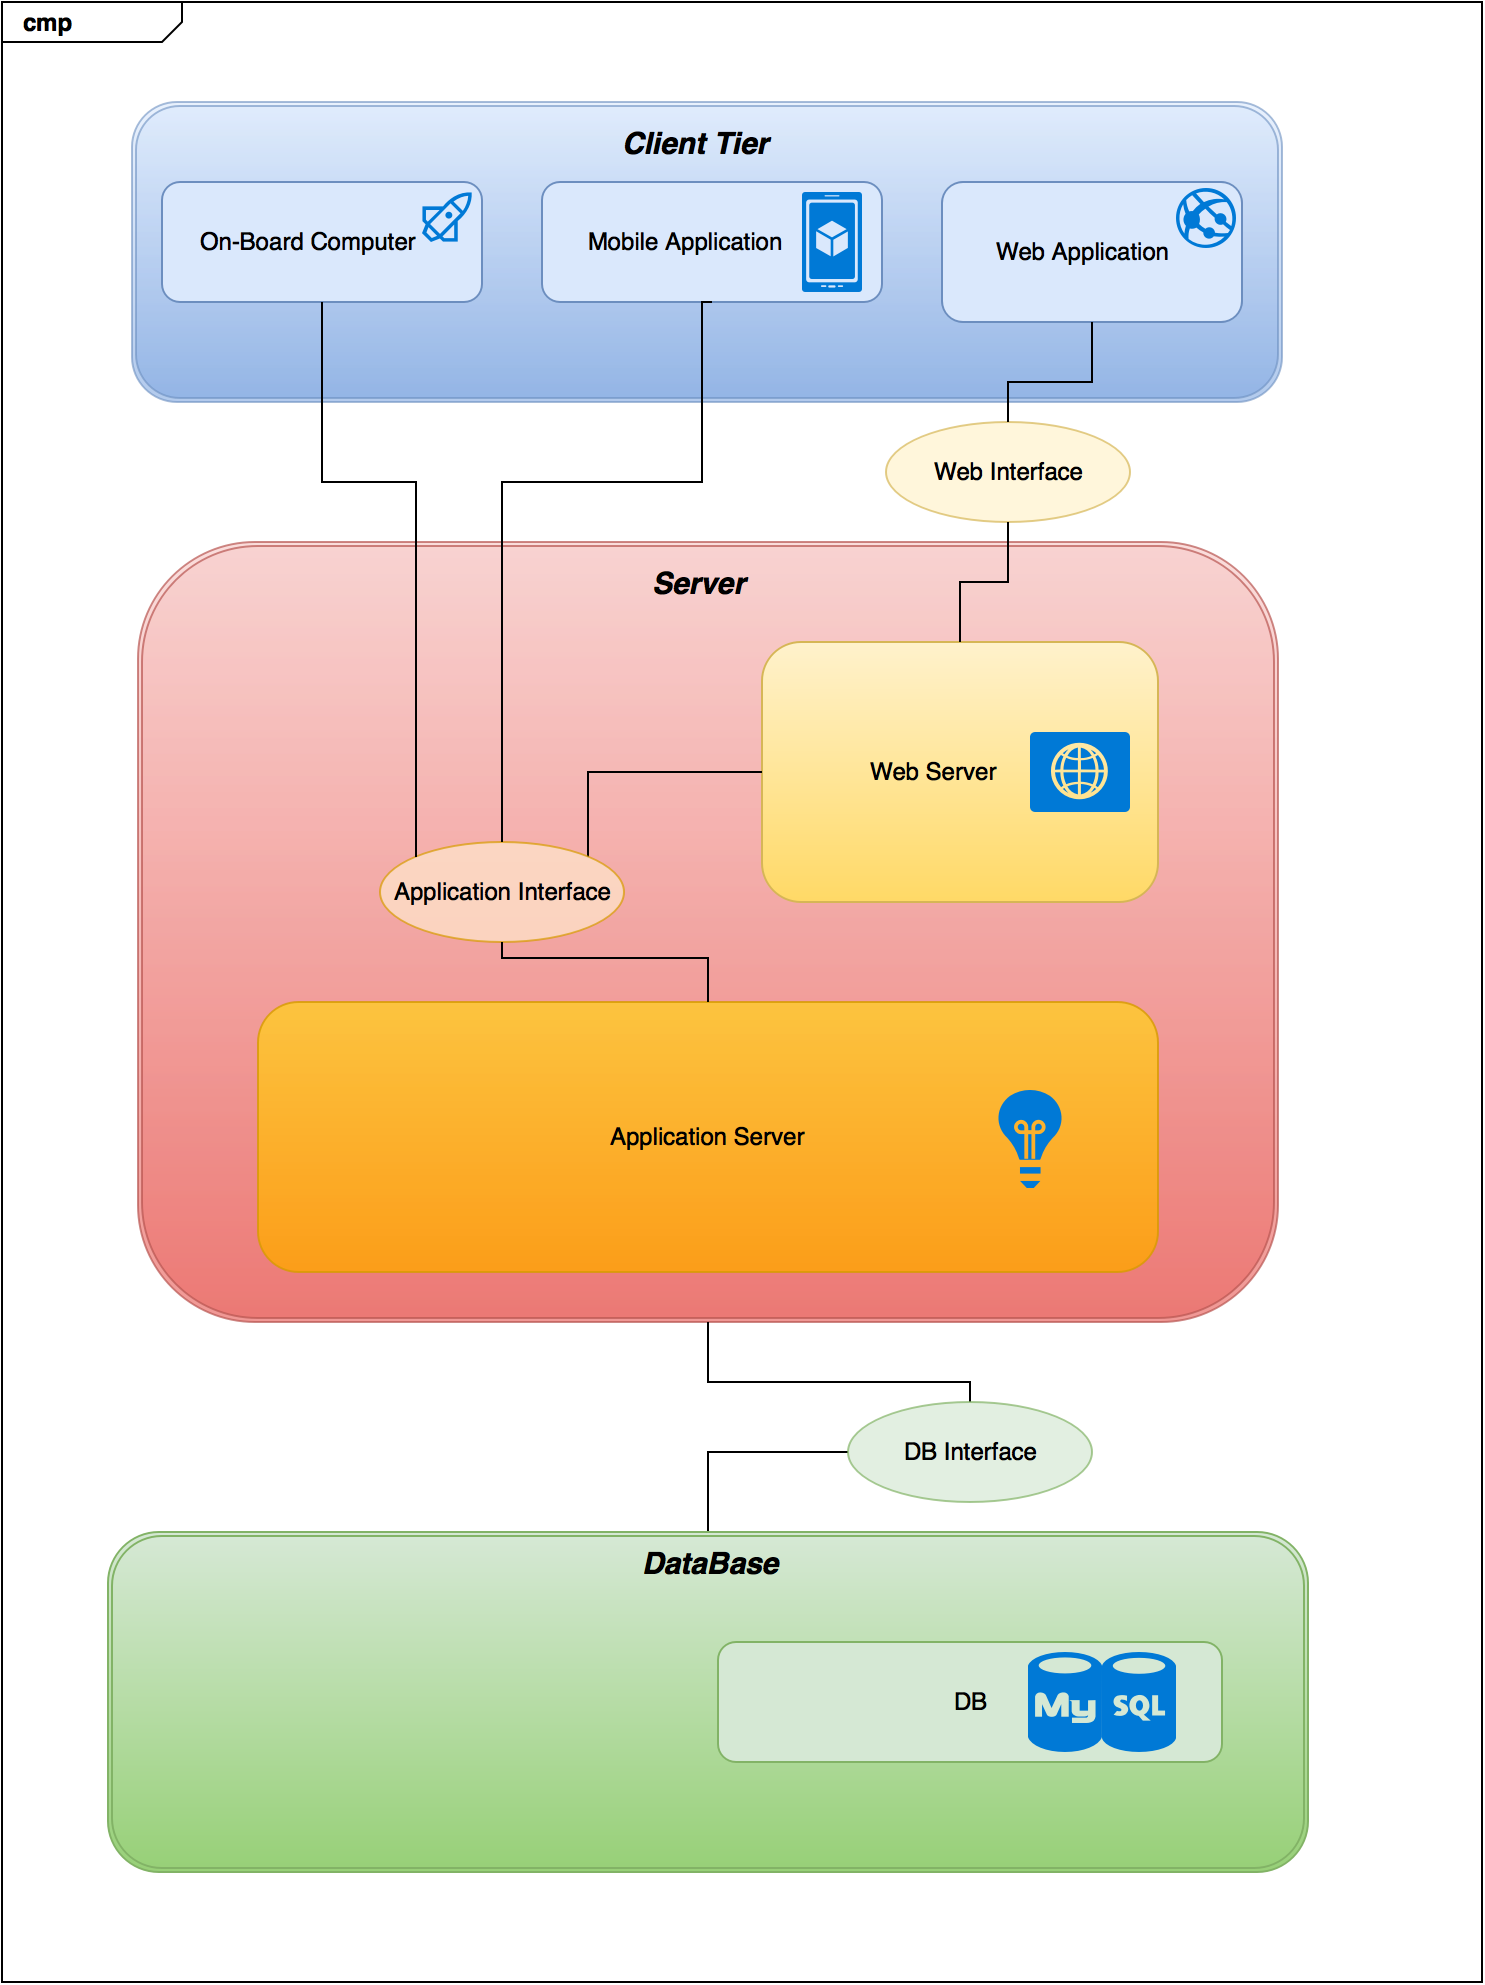
\includegraphics[width=0.6\textwidth]{/DD/4-Tier_Architecture}\\
  \vspace{0.4cm}
  \caption{Components Diagram} 
  \label{fig:4-Tier_Architecture} 
\end{figure}

This represent a high level view of the design of the system, were is highlighted the distribution of the system over the three locations and the interaction between the different tiers thanks to their interfaces.
\\The Client Tier is composed by the On-board computer, the mobile application and the web application.
\\The Web Tier and the Business Tier are inside the server machine. We can observe that the Web application need to interact with the Web Server before to access to the Application server while the mobile application has a direct access to it.
\\The EIS Tier consists in a database that store all the system's data and interact through the DB Interface with the server.

 \section{Component view}
\subsection{System components}
To define and easily understand what kind of functionalities must be implemented in our system we decided to decompose PowerEnJoy logically into components. Then it is analysed each component and the interaction that it has with the other components, so the common parts can be identified if present. The components are studied to be reusable and easily adaptable in other applications.
%We have decided to decompose PowerEnJoy in different components in order to make it easy to understand what kind of functionalities must be implemented and to separate them, logically, in groups, to state clearer their interaction. The analysis of each component will give us the possibility to find common parts, if there are, and reuse them. 
\\The identified components are:
\begin{itemize}
	\item Access functionalities: provide sign-up to guests and log-in to users. They also allow credentials retrieving.
	\item Profile functionalities: provide the possibility for an user to modify her personal information.
	\item Reservation of the car: this functionality allows users to localize and reserve an available car.
	\item Ride functionalities: provide the possibility to unlock and lock of the car. Then all the system functions related with the ride are allocated here. %to change???
	\item Notification functionalities: provide the visualization of users' notifications, related to payments and reservations.%something else?
	\item Payments functionalities: provide the application of discounts or fees to a ride and menage the process related with the payments.
\end{itemize}

\subsection{Database components}
In particular the data stored in the database will be split through different subcomponents that identified the main entities of our system:
User,Vehicle, Location, Safe Area, Charging Station, Reservation, Ride, Behaviours and Payment.  
\\The designed model for persistent data is provided here in a ER diagram in order to better analyze the motivations of our design. That's the representation of the database model:
\begin{figure}[!h]
  \centering
  \vspace{0.2cm}
  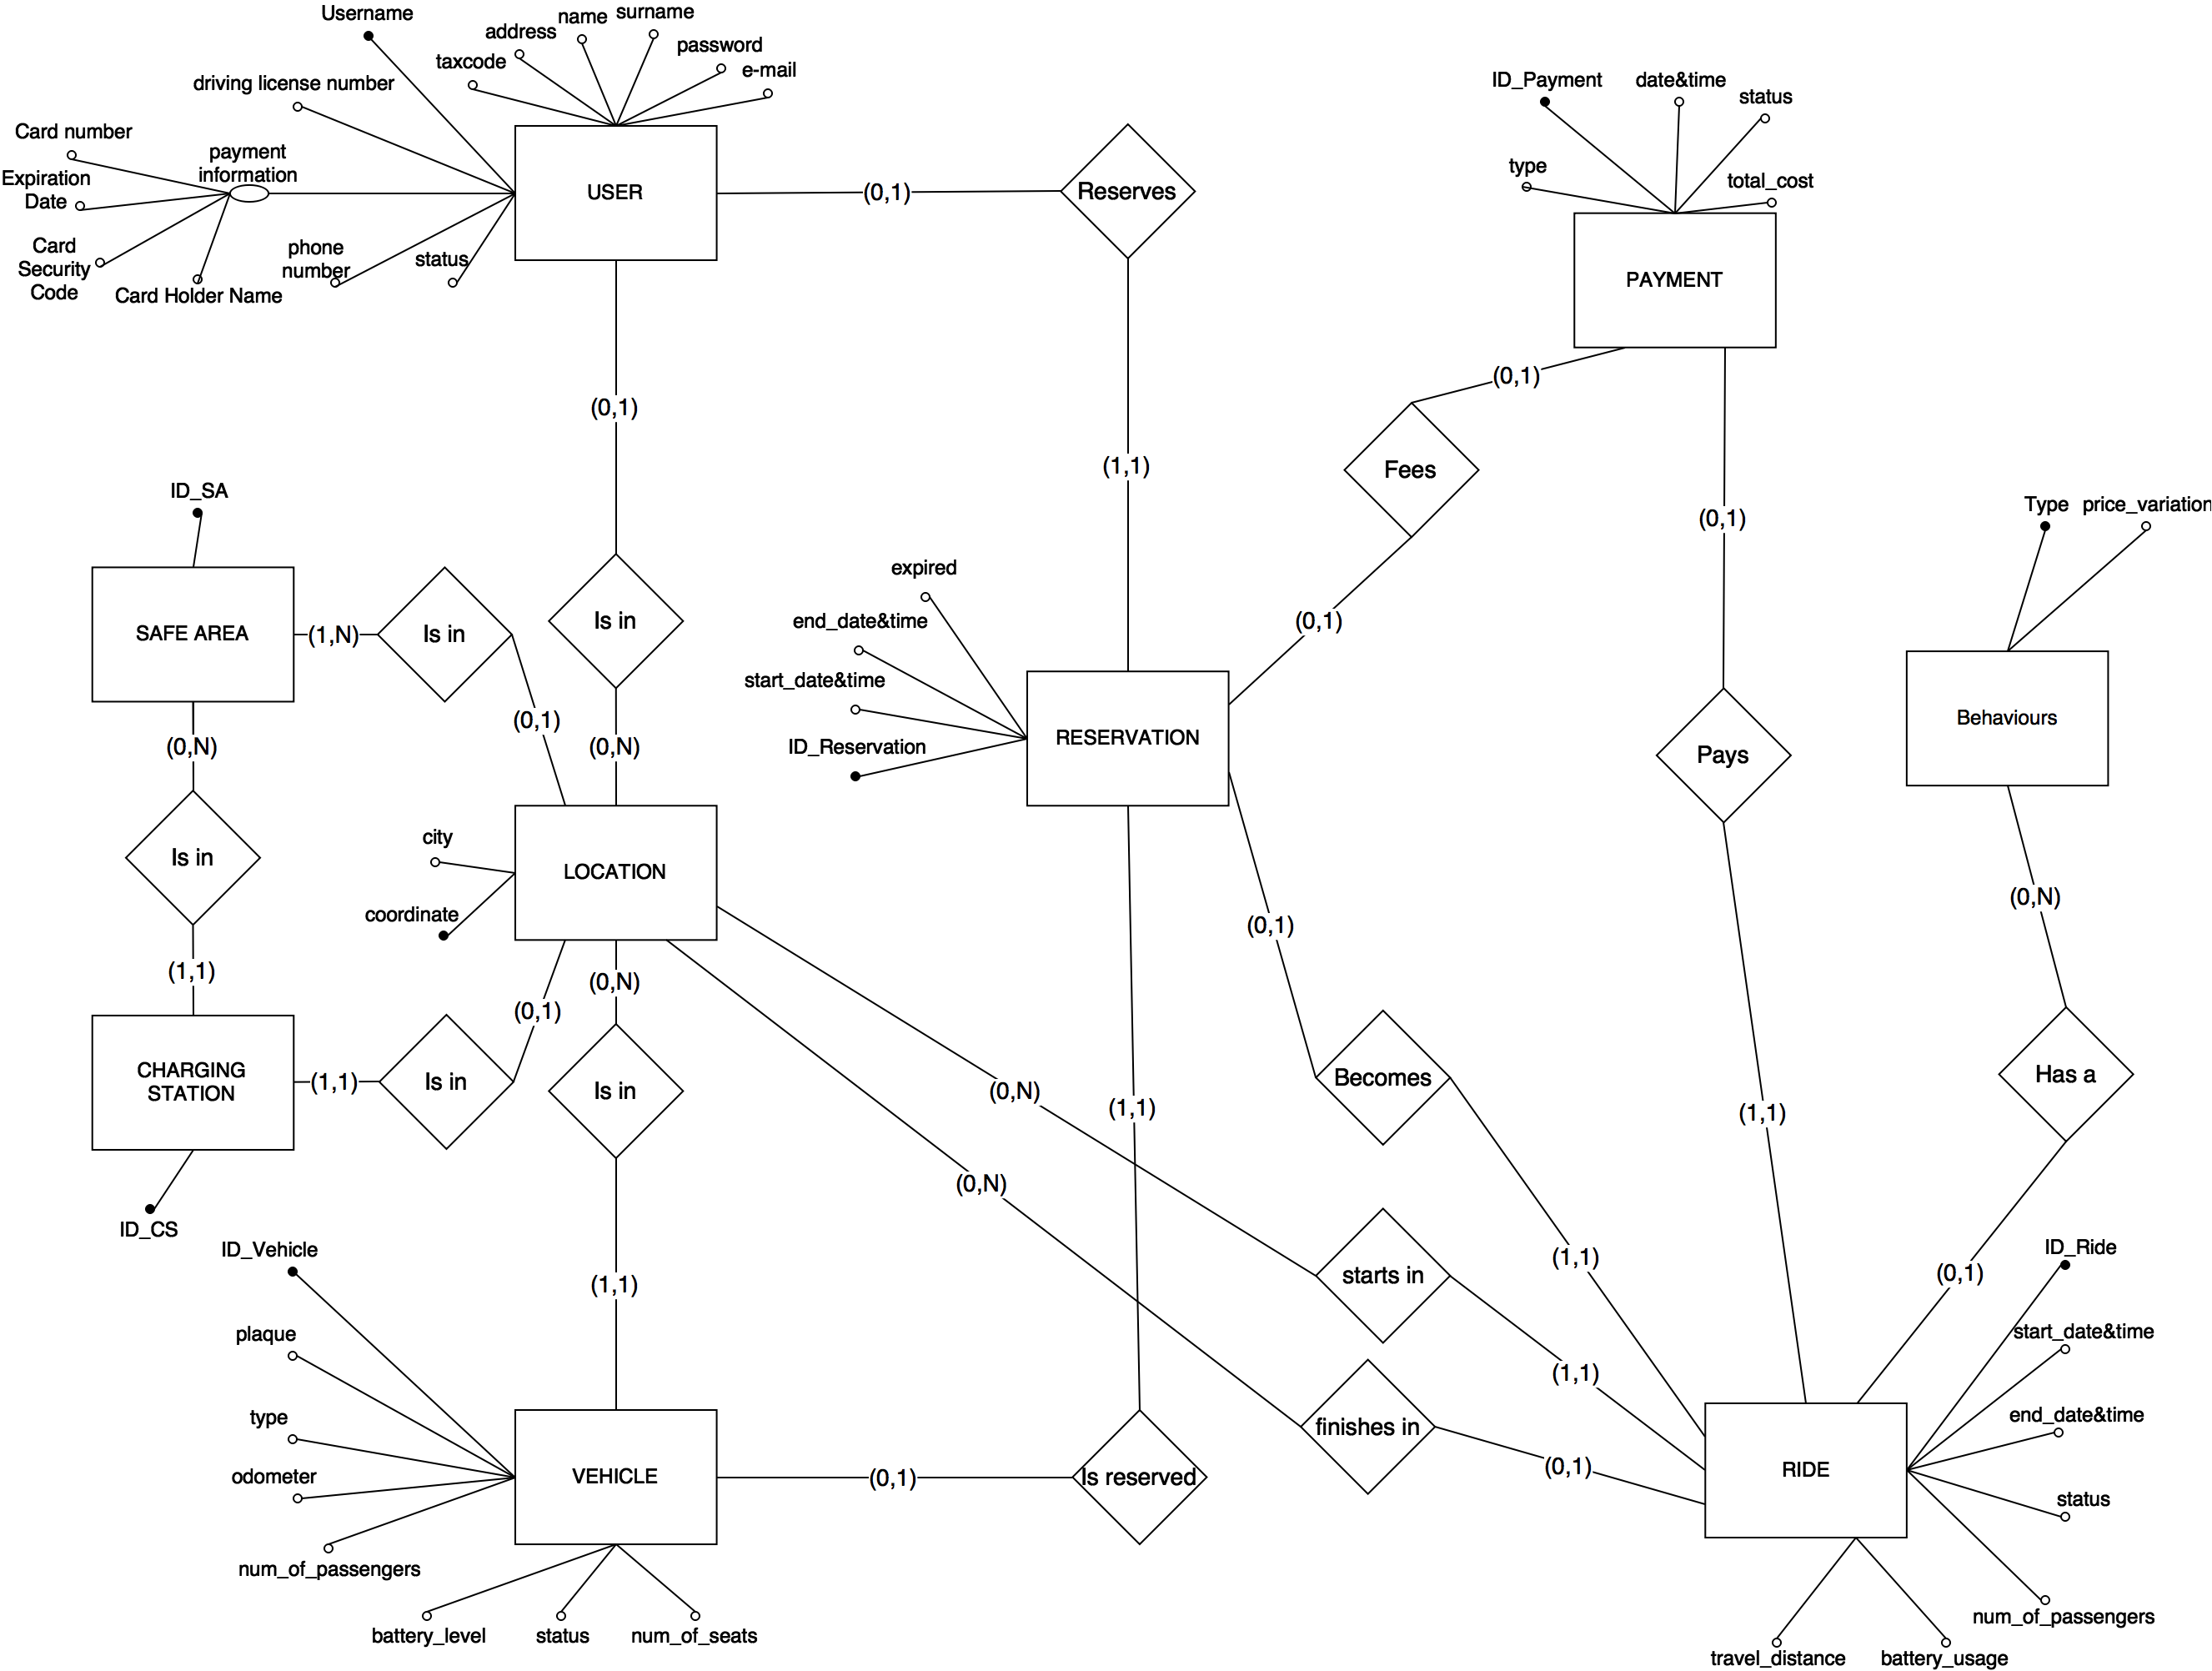
\includegraphics[width=0.7\textwidth]{/DD/ER_Diagram}\\
  \vspace{0.4cm}
  \caption{ER Diagram} 
  \label{fig:ER_Diagram} 
\end{figure}

 And this is the relation schema associated with the ER diagram.
\begin{itemize} 
	\item{User (\underline{Username}, \textit{Location}, e-mail, password, driving\_license\_number, name, surname, address, phone number, taxcode, card\_number, expiration\_date, card\_security\_code, card\_holder\_name, status)} %status: reserving, riding, free, (guarda caso utente bloccato)
	\item{Vehicle (\underline{ID\_Vehicle}, \textit{Location}, plaque, type, odometer, battery\_level, status, num\_of\_seats, num\_of\_passengers) }
	\item{Location (\underline{coordinate}, city)}	
	\item{Safa Area (\underline{ID\_SA}, \textit{Location})} %type A=Safe Area, B=Charging Station, C=both, Add an ID!!!
	\item{Charging Station(\underline{ID\_CS}, \textit{Location})}
	\item{Reservation (\underline{ID\_reservation}, \textit{ID\_User}, \textit{ID\_Vehicle}, reservation\_date\&time, unlock\_date\&time, expiration\_date\&time, status)}
	\item{Ride (\underline{ID\_Ride}, \textit{ID\_User}, \textit{ID\_Vehicle}, \textit{ID\_Reservation}, \textit{ID\_Payment},\textit{Start\_Location},\textit{Finish\_Location}, start\_date\&time, end\_date\&time, status, num\_of\_passengers, travel\_distance, battery\_usage)}
	\item{Behaviours(\underline{Type}, \textit{ID\_Ride}, price\_variation)}
	\item{Payment (\underline{ID\_Payment}, \textit{ID\_User}, \textit{ID\_Reservation}, \textit{ID\_Ride}, date\&time, total\_cost, status, type)}
\end{itemize}
In the User entity there are all the main information about the user such as credentials and payment method. Her status can be reserving, riding, free or banned. The location of the user is not necessary.
\\A Vehicle entity has different attributes, some of them supply by the On-Board computer. The status here can be free, reserved, in_use or out_of_order.
\\The Location entity represent a location provided by the GPS. Safe area are zones composed by one or more locations. Into the Safe areas there can be also some Charging stations.
\\The Reservation entity is connected with an user and a vehicle. It can end or with an unlock or with an expiration, and in this second case it comports the payment of a fee by the user. The reservation is strictly connected with the Ride entity, which can exist only related with it. Each ride has a starting point and when it finishes an end point. A ride also comports a payment, in particular if the Behaviours entity is present related with the ride it comport a variation of the final price. 
\\In the Payment entity there are the information about the transaction from th user to PowerEnJoy, the status indicates if the payments has been done with success or if the system is still waiting for it.

\section{Deployment view}
The hardware topology is described here, highlighting components and their relationships. The software parts are deployed in or-
der to have the system working.
\\As previously see in the Overview the system will run thanks of 4 main components:
\begin{itemize}
	\item{The client device, where an User can interact with the system. There are different GUI that renders the web or mobile pages of our system, differentiating between On-board computer, mobile application and web application.}
	\item{ The Web Server is needed for those who are connected to the system with a computer. It establishes a secure internet connection through the HTTPS protocol.}
	\item{The Application Server is the core of our system. Here we have the Business Logic, where the whole system computation is
made.}
	\item{In the Database all the information of the system are stored. It's accessible only by the Application Server that store and take data from there.}
\end{itemize} 

\begin{figure}[!h]
  \centering
  \vspace{0.2cm}
  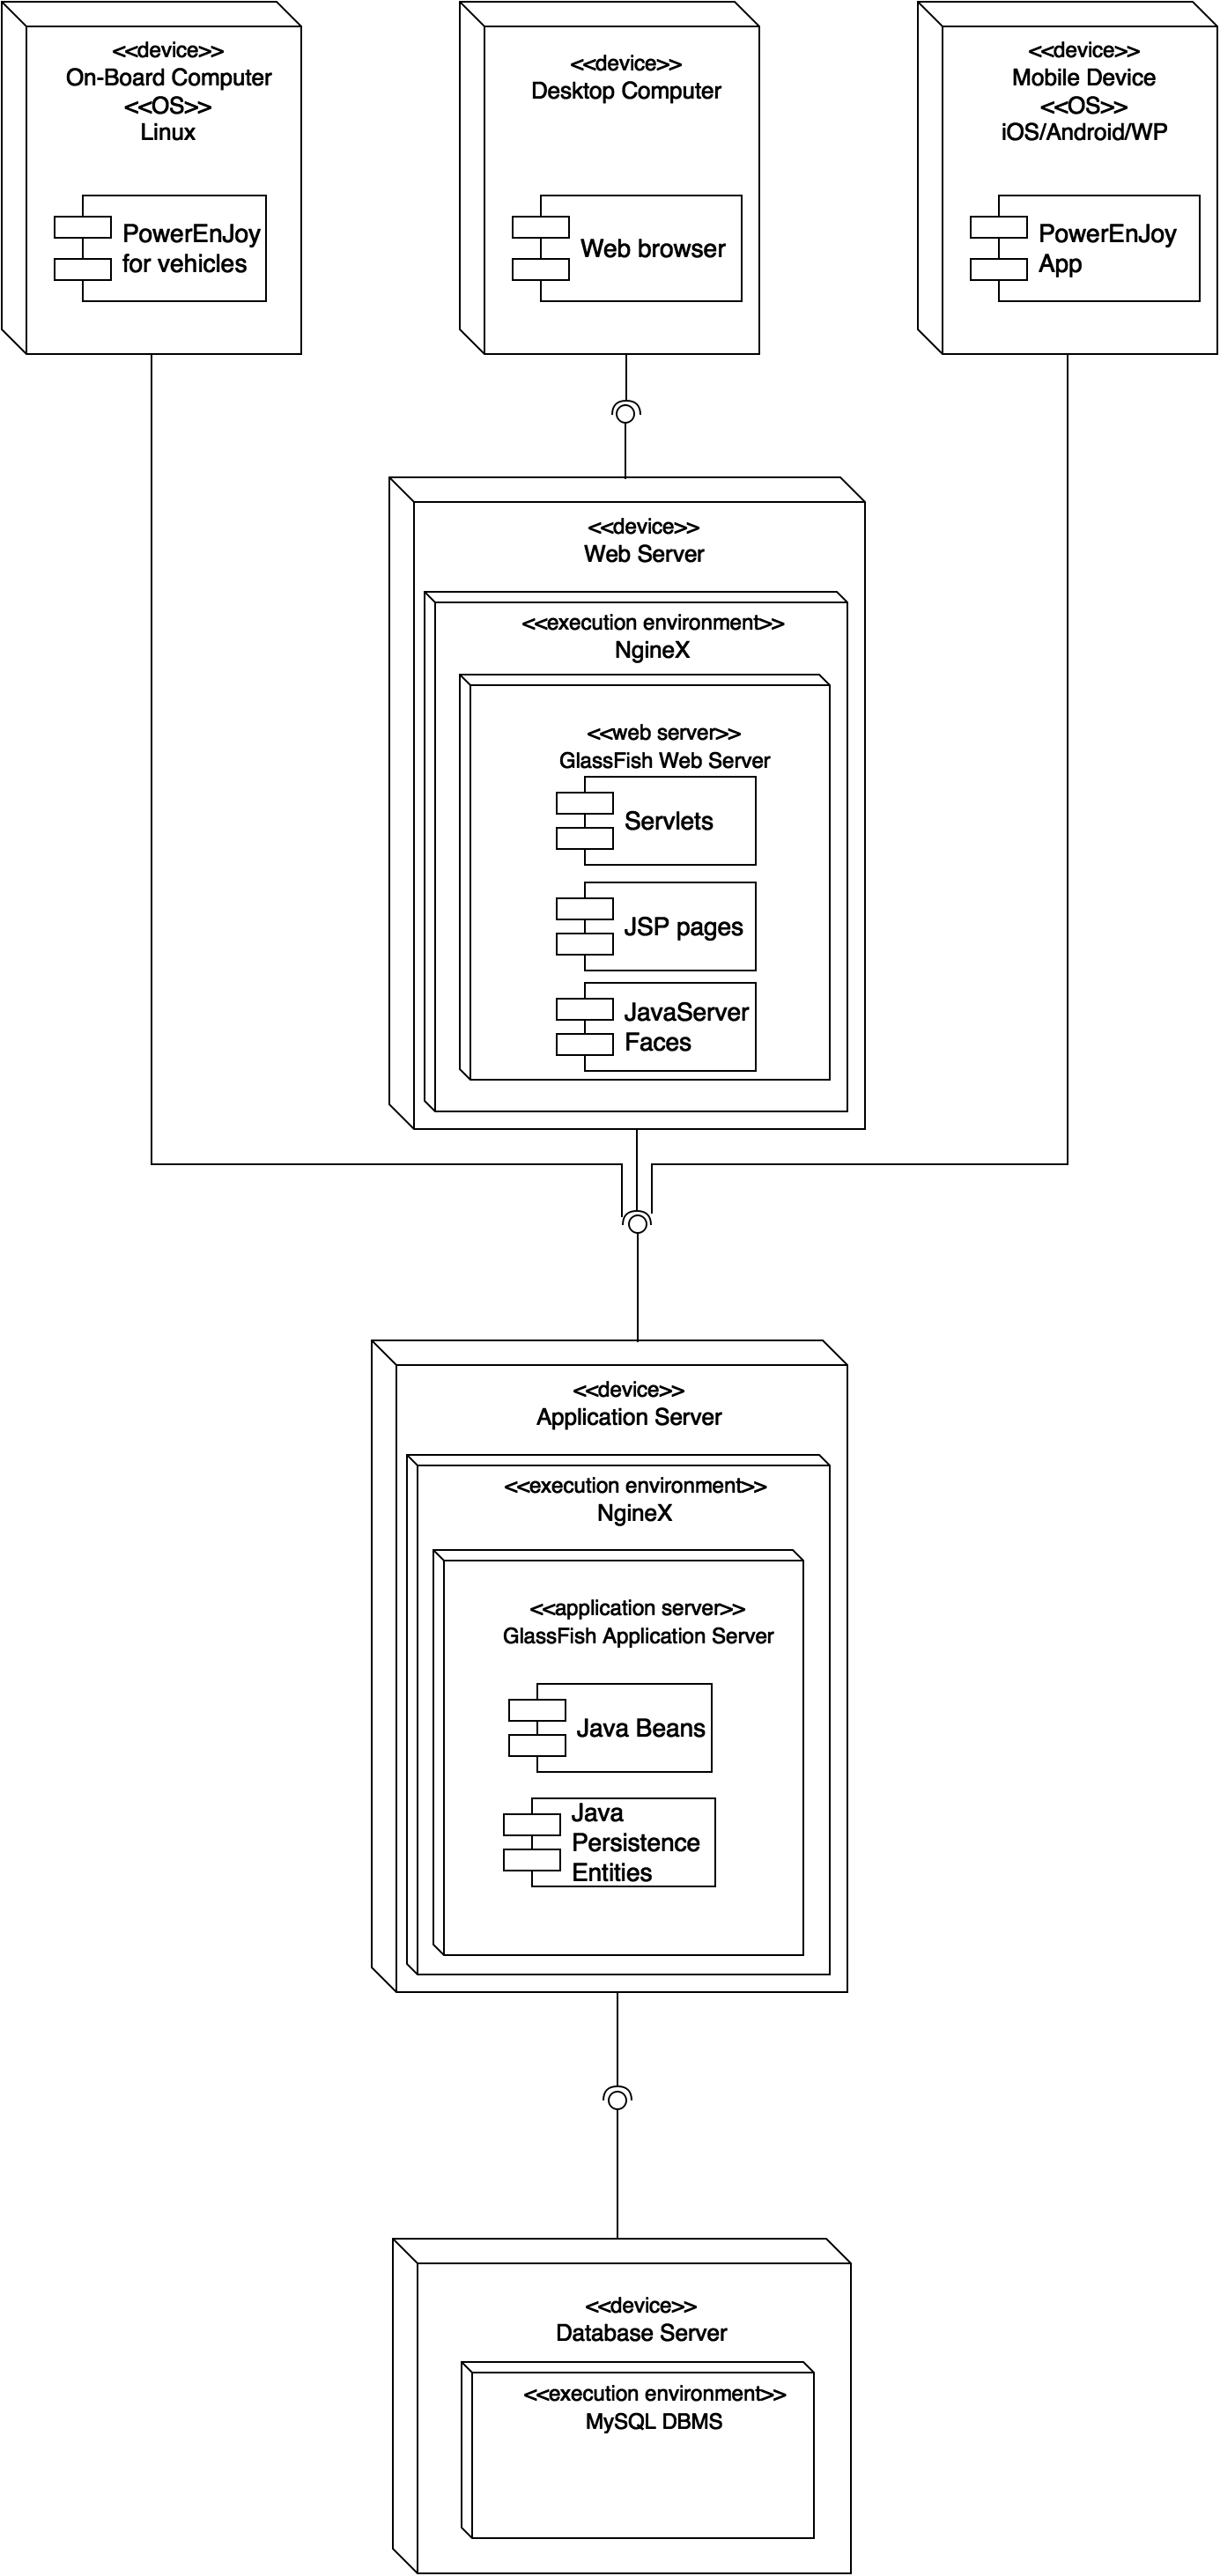
\includegraphics[width=0.6\textwidth]{/DD/DeploymentView}\\
  \vspace{0.4cm}
  \caption{Components Diagram} 
  \label{fig:Deployment View} 
\end{figure}


\section{Runtime view}

In order to state the interaction between the different components of the system here are presented some sequence diagrams.
\\The sequence diagrams highlight the part of the system that interact for implement a function and the messages exchanged between them.



 \section{Component Interfaces}
 	\blindtext
%Questo e' copiato da quello dello scorso anno.
\begin{comment}
 PDO: PHP Data Objects used by the BLL to communicate with the DAL.
 	RESTful API with JSON used by clients ( both mobile apps and web
browsers ) to interact with the BLL. API calls that need authentication are
required to authenticate via HTTP basic authentication for each request. exchanged
data will be secured using SSL.
as now ( v1 ) our exposed methods are the following:
• api/v1/driver [auth]
– GET: get driver info
– PATCH/PUT: update driver data ( position and available status )
• api/v1/request
– POST: create a new request
• api/v1/reservation
– POST: create a new reservation
• api/v1/ride
– POST: create a new ride
\end{comment}

 \section{Selected architectural styles and patterns}
Building this application different architectural styles and patterns have been used.
\subsection{4-tier JEE client-server architecture}
	This archtectural style has been used for separating efficiently the different levels of execution. The components of the application are identified in this tiers:
	\begin{itemize}
		\item{Client tier: is the layer that interact with the users. It runs on the client machine. This layer contains the On-Board computer, the Mobile application and the Web application.}
		\item{Web tier: is the layer that manage the interaction between the Web application and the Business tier. It contains Servlets, JSP pages and JavaServer Faces. In our system it is implemented by the Web server.}%giusto definire cosi' la cosa?
		\item{Business tier: contains Java Beans and Java Persistence Entities. It receives data from client programs, processes it (if necessary), and sends it to the enterprise information system tier for storage. An enterprise bean also retrieves data from storage, processes it (if necessary), and sends it back to the client program. In our system it is implemented by the Application server.}
		\item{Enterprise Information System tier: runs EIS software and includes enterprise infrastructure systems, such as enterprise resource planning (ERP), mainframe transaction processing, database systems, and other legacy information systems. It represents the data layer. The MySQL Database server is chosen for the creation and the maintainance of all the application data.}
	\end{itemize}
	\begin{figure}[!h]
  \centering
  \vspace{0.2cm}
  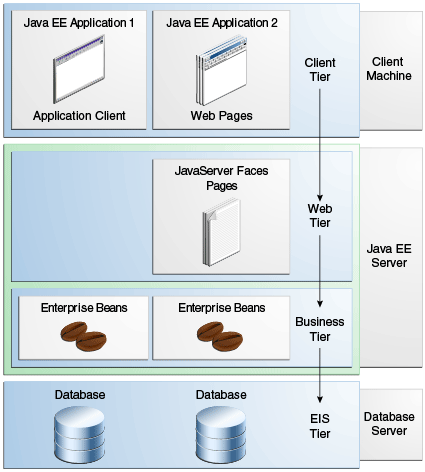
\includegraphics[width=0.6\textwidth]{/DD/Architecture_of_the_system}\\
  \vspace{0.4cm}
  \caption{Components Diagram} 
  \label{fig:Architecture of the system} 
\end{figure}
\subsection{Client-Server}
	The client-server communication model is highly used in this application.
	The On-Board computer and the Mobile application are clients with respect to the Application Server. The Web application consist of a Web browser that is a client with respect to the Web Server. The Web server is also a client with respect to the Application server. The Database is a server with respect to the Application server that act as a client.
\subsection{Thin client}
	In order to avoid that the client machine is involved in any logic decision we decided that all the computations will be run in the Application server. This comports different important advantages for the client tier: the client application will comport lower operational cost for the device, a superior security is obteined, the data are synchronizated and the sistem is highly reliable. In addition this make the application indipendent from the number of clients connected.
\subsection{MVC}
	The Model-View-Controller pattern has been used in this application during the implementation of the client tier. In this way we separated the model, that rapresent the knowledge, the view, that is a visual rapresentation of the model, and the controller, that is the link between a user and the system.

 \section{Other design decisions}
 	\blindtext